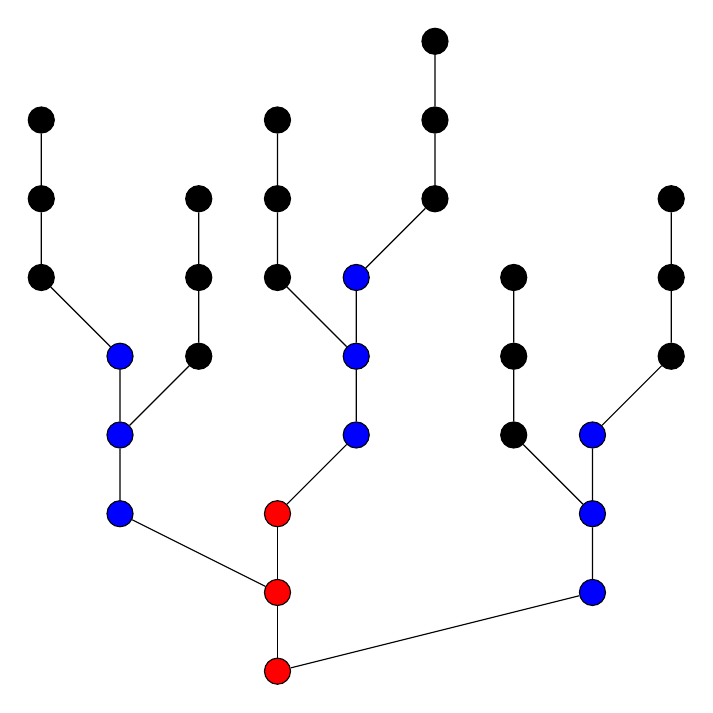
\begin{tikzpicture}[every node/.style={draw,shape=circle,fill=black}]

\node[fill=red] (A) at (0,0) {};
\node[fill=red] (B) at (0,1) {};
\node[fill=red] (C) at (0,2) {};

\draw (A) -- (B) (B) -- (C);

\node[fill=blue] (D) at (4,1) {};
\node[fill=blue] (E) at (4,2) {};
\node[fill=blue] (F) at (4,3) {};

\draw (A) -- (D) (D) -- (E) (E) -- (F);

\node[fill=blue] (G) at (-2,2) {};
\node[fill=blue] (H) at (-2,3) {};
\node[fill=blue] (I) at (-2,4) {};

\draw (B) -- (G) (G) -- (H) (H) -- (I);

\node[fill=blue] (J) at (1,3) {};
\node[fill=blue] (K) at (1,4) {};
\node[fill=blue] (L) at (1,5) {};

\draw (C) -- (J) (J) -- (K) (K) -- (L);

\node (P) at (-1,4) {};
\node (Q) at (-1,5) {};
\node (R) at (-1,6) {};

\draw (H) -- (P) (P) -- (Q) (Q) -- (R);

\node (S) at (-3,5) {};
\node (T) at (-3,6) {};
\node (U) at (-3,7) {};

\draw (I) -- (S) (S) -- (T) (T) -- (U);

\node (V) at (0,5) {};
\node (W) at (0,6) {};
\node (X) at (0,7) {};

\draw (K) -- (V) (V) -- (W) (W) -- (X);

\node (Y) at (2,6) {};
\node (Z) at (2,7) {};
\node (AA) at (2,8) {};

\draw (L) -- (Y) (Y) -- (Z) (Z) -- (AA);

\node (AE) at (3,3) {};
\node (AF) at (3,4) {};
\node (AG) at (3,5) {};

\draw (E) -- (AE) (AE) -- (AF) (AF) -- (AG);

\node (AH) at (5,4) {};
\node (AI) at (5,5) {};
\node (AJ) at (5,6) {};

\draw (F) -- (AH) (AH) -- (AI) (AI) -- (AJ);

\end{tikzpicture}